\chapter{Meta}

\section{Hintergrund}

Section Hintergrund

\section{Namensherkunft}

Der Name \textbf{Shulker} stammt ursprünglich aus der dem Videospiel \textit{Minecraft}. In Minecraft ist ein Shulker eine Kreatur, die Verschlossen ist.

\begin{figure}[H]
    \begin{center}
        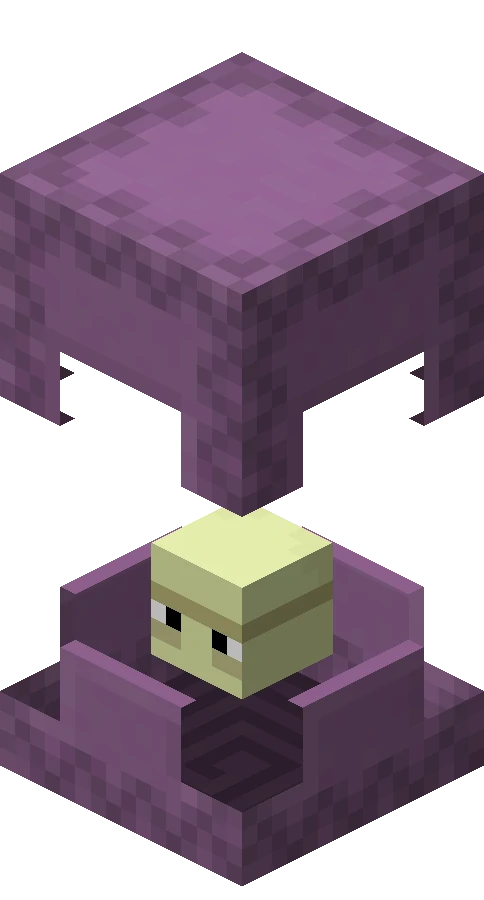
\includegraphics[width=0.22\textwidth]{images/Intro/Shulker.png}
        \caption{Die Kreatur \textbf{Shulker} aus dem Videospiel \textit{Minecraft}}
        \cite{mcwiki2015}
    \end{center}
\end{figure}

\newpage

\section{Projektlogo}

Text über das Projektlogo